\begin{frame} % Слайд 1
    \begin{center}
        \small
        Волгоградский Государственный Технический Университет \\
        Факультет электроники и вычислительной техники \\
        Кафедра САПРиПК \\
        \vspace{1.5cm}
        \normalsize
        \textbf{Метод построения маршрутов общественного транспорта на основе 
        предпочтений жителей.}\\
        \vspace{1.0cm}
        \raggedleft\small
        \textbf{Исполнитель:}\\Голубев~А.~В.\\
        \textbf{Руководитель:}\\Щербаков~М.~В.\\
        \vspace{1.5cm}
        \vspace{\fill}
        \centeringВолгоград \the\year
    \end{center}
\end{frame}

\begin{frame} % Слайд 2
    \frametitle{Формулировка проблемы}
    \textbf{Актуальность.} Изменения в городской среде требуют формирования новых 
    механизмов планирования инфраструктуры города. Для получения эффективных 
    результатов, следует осуществлять принятие решений на основе актуальных 
    данных, отражающих предпочтения жителей.\\
    \textbf{Объект исследования} -- построения маршрутов общественного транспорта.\\
    \textbf{Предмет исследования} -- методы построения маршрутов учитывающие предпочтения жителей.
\end{frame}

\begin{frame} % Слайд 3
    \frametitle{Цели и задачи}
    \textbf{Цель работы} -- разработка метода генерации маршрутов общественного 
    транспорта на основе предпочтений жителей для минимизации дискомфорта 
    перемещения в городе. \\
    \textbf{Теоретические задачи:}
    \begin{itemize}
        \item разработка алгоритма обхода кластеров;
        \item построение маршрута по заданным критериям;
        \begin{itemize}
            \item предпочтения жителей;
            \item длина маршрута;
            \item и д.р.
        \end{itemize}
        \item разработка критериев для оценки качества построенного маршрута;
    \end{itemize}
    \textbf{Практические задачи:}
    \begin{itemize}
        \item генерация исходных данных;
        \item реализация разработанных алгоритмов и методов;
        \item построение полученных маршрутов на карте;
        \item оценка качества построенных маршрутов.
    \end{itemize}
\end{frame}

\begin{frame} % Слайд 4
    \frametitle{Понятийный аппарат}
    \small
    \begin{itemize}
        \itemsep-5pt
        \item \textbf{граф} -- совокупность непустого множества вершин и наборов пар вершин;
        \item \textbf{ребро графа} -- линия, соединяющая пару смежных вершин графа; 
        \item \textbf{узел графа} -- вершина графа;
        \item \textbf{кластер} -- объединение нескольких однородных элементов, которое может 
            рассматриваться как самостоятельная единица, обладающая определёнными свойствами;
        \item \textbf{node (точка)} -- точка с указанными координатами;
        \item \textbf{way (линия)} -- упорядоченный список точек, составляющих линию или полигон;
        \item \textbf{relation (отношение)} -- группы точек, линий и других отношений, которым назначаются 
            некоторые свойства;
        \item \textbf{tag (тег)} -- пары <<ключ -- значение>>, могут назначаться точкам, линиям и отношениям.
    \end{itemize}
\end{frame}

\begin{frame} % Слайд 5
    \frametitle{Список литературы}
    \begin{itemize}
        \item Route Planning in Transport Networks\\
            \tiny\url{http://research.microsoft.com/pubs/207102/MSR-TR-2014-4.pdf}
        \item\normalsize Online Graph Pruring for Pathfinding on Grid Maps
            \tiny\url{http://users.cecs.anu.edu.au/~dharabor/data/papers/harabor-grastien-aaai11.pdf}
        \item\normalsize Contraction Hierarchies: Faster and Simpler Hierarchical 
            Routing in Road Networks\\
            \tiny\url{http://algo2.iti.kit.edu/schultes/hwy/contract.pdf}
        \item\normalsize Генетические алгоритмы\\
            \tiny\url{http://mathmod.aspu.ru/images/File/ebooks/GAfinal.pdf}
        \item\normalsize Генетический алгоритм для определения минимального времени пути в 
            интеллектуальных транспортных система\\
            \tiny\url{http://masters.donntu.org/2010/fknt/kazakovaj/library/translate1.htm}
        \item\normalsize Алгоритмы решения задачи быстрого поиска пути на географических картах\\
            \tiny\url{http://engjournal.ru/articles/1054/1054.pdf}
        \item\normalsize Поиск кратчайших путей на графе дорог\\
            \tiny\url{http://mit.spbau.ru/files/kononenko.pdf}
    \end{itemize}
\end{frame}

\begin{frame} % Слайд 6
    \frametitle{Прототип}
    Псевдокод поглощающего алгоритма:\\
    \begin{figure}
        \begin{minipage}{0.6\textwidth}
            \tiny
            \textbf{ВВОД} количество\_маршрутов, максимальная длина\\
            \textbf{ДЕЛАТЬ ПОКА} маршрут < количество\_маршрутов:\\
                \hspace*{0.5cm}\textbf{НАЙТИ} ребро графа с максимальной потребностью\\
                \hspace*{0.5cm}\textbf{ВЫБРАТЬ} вершину с большим числом людей\\
                \hspace*{0.5cm}\textbf{ДЕЛАТЬ ПОКА} длина != максимальная\_длина:\\
                    \hspace*{1.0cm}\textbf{ВЫБРАТЬ} ребро с максимальной потребностью\\
                    \hspace*{1.0cm}\textbf{ПЕРЕЙТИ} в вершину\\
                    \hspace*{1.0cm}длина += 1\\
                \hspace*{0.5cm}маршрут += 1\\
        \end{minipage}
        \begin{minipage}{0.37\textwidth}
            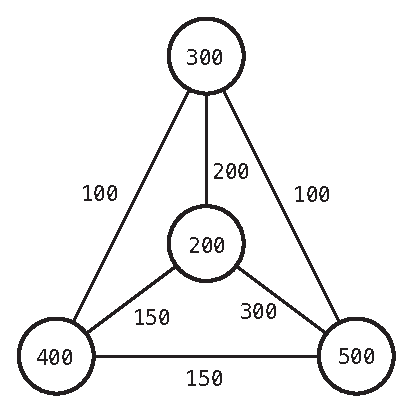
\includegraphics[width=\textwidth]{img01}
        \end{minipage}
    \end{figure}
\end{frame}

\begin{frame} % Слайд 7
    \frametitle{Прототип}
    \begin{figure}
        \begin{minipage}{0.47\textwidth}
            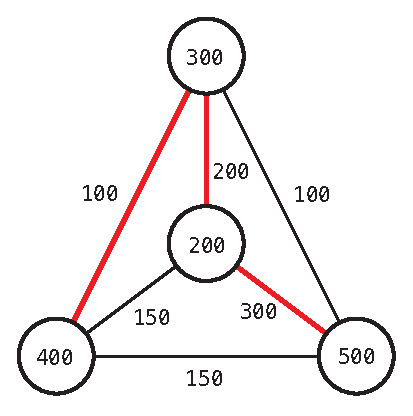
\includegraphics[width=\textwidth]{img02}
        \end{minipage}
        \begin{minipage}{0.47\textwidth}
            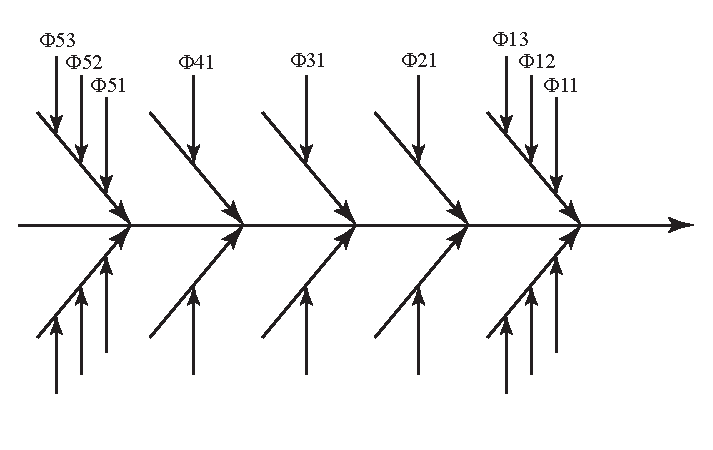
\includegraphics[width=\textwidth]{img03}
        \end{minipage}
    \end{figure}
    \small\emph{Реализованный алгоритм:} \url{https://github.com/FreeCX/cluster-routing}\\
\end{frame}

\begin{frame} % Слайд 8
    \frametitle{Результат}
    \begin{figure}
        \center
        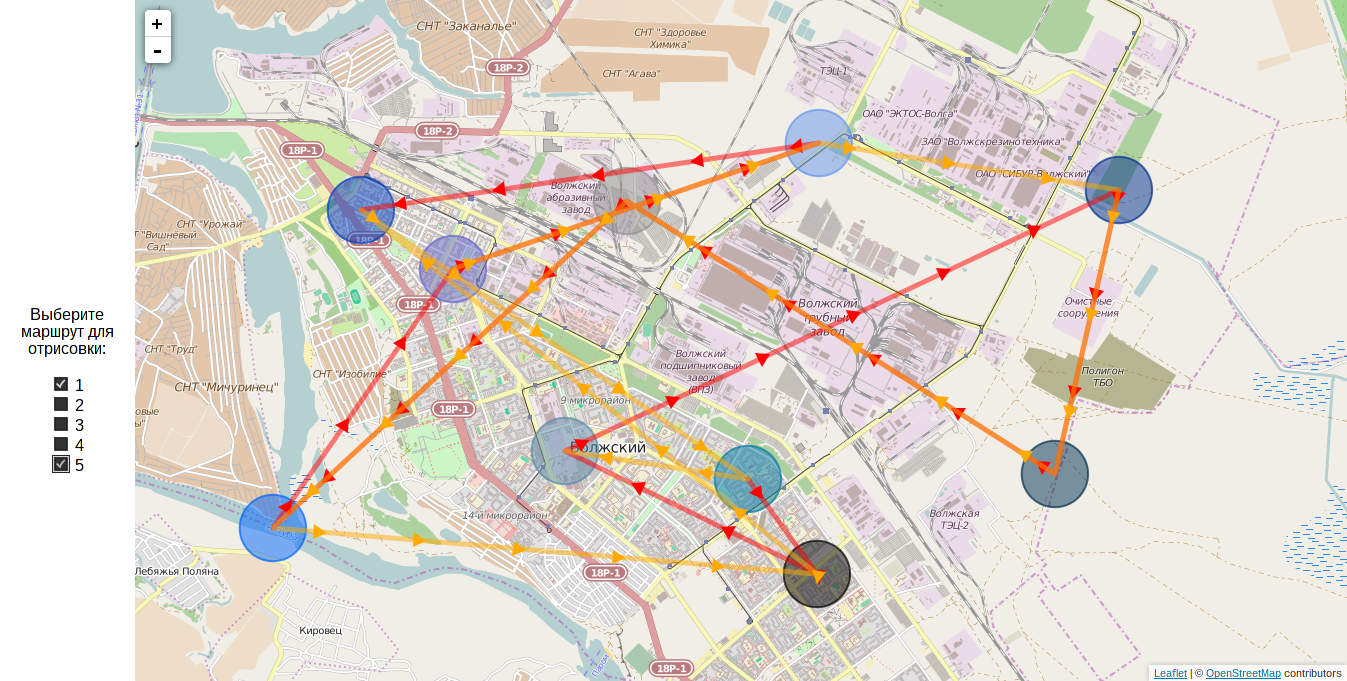
\includegraphics[width=\textwidth]{routing}
    \end{figure}
    \small\emph{Ссылка на результат работы алгоритма:} \url{http://freecx.github.io/routing/}
\end{frame}